\documentclass[10pt]{beamer}
\usepackage{verbatim}
\usepackage{amsmath}
\usepackage{amsthm}
\usepackage{graphics}
\usepackage{color}
\usepackage{algorithm, algorithmic}
\usepackage{stmaryrd}\usefonttheme[onlymath]{serif}

\title{Discussion 5: Experiment Results \& Tool Demo}
\begin{document}

\maketitle
\begin{frame}\frametitle{Experiment Results}
\textbf{General Result: }
\begin{center}
\begin{tabular}{|c|c|c|c|c|}
\hline
& 2-Multiphase& 5-Multiphase & SVMRanker & LassoRanker\\
\hline 
FINITE & 39 & 42&30 & 24\\
\hline 

INFINITE & 34& 34&34 & 37\\
\hline

UNKNOWN & 61& 58&70 & 73\\
\hline
TIME &1107s& 5709s& 162s& 1695s\\
\hline

\end{tabular}
\end{center}


\end{frame}


\begin{frame}\frametitle{Experiment Results}
\textbf{Time Details:}

\begin{center}
\begin{tabular}{|c|c|c|c|}
\hline
& 2-Multiphase& 5-Multiphase & SVMRanker\\
\hline 
sampling &79.6s & 472.0s & 11.6s \\
\hline
training & 52.4s & 396.7s& 4.8s\\
\hline 
z3-solving & 229.2s& 4016.1s& 22.6s\\
\hline
\end{tabular}
\end{center}

\end{frame}

\begin{frame}\frametitle{Experiment Results}
\textbf{Examples in SV-COMP15/Mumeric \& Crafted:}

\begin{center}
\begin{tabular}{|c|c|c|c|c|}
\hline
& 2-Multiphase& 5-Multiphase & SVMRanker\\
\hline 
FINITE & 22 & 22& 20\\
\hline 

INFINITE & 7& 7& 7\\
\hline

UNKNOWN & 23& 23& 25\\
\hline

\end{tabular}
\end{center}

\end{frame}

\begin{frame}\frametitle{Experiment Results}
\textbf{Num of linear and non-linear loops}
\begin{center}
\begin{tabular}{|c|c|c|c|c|}
\hline
 & 2-Multiphase& 5-Multiphase & SVMRanker & LassoRanker\\

 
\hline
linear &   21 & 23 & 14 & 22\\
\hline 
non-linear &  18& 19 & 16 & 2\\
\hline
\end{tabular}
\end{center}
\end{frame}

\begin{frame}\frametitle{Tool Demo}
\begin{center}
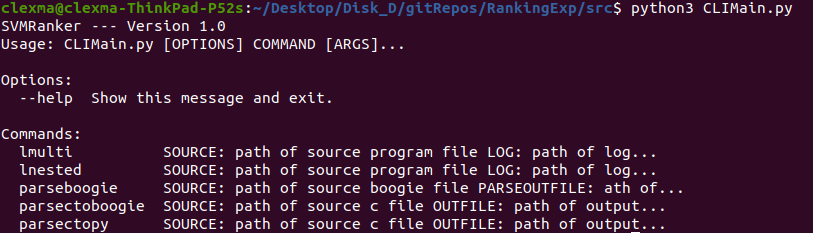
\includegraphics[scale=0.4]{1.png}
\end{center}

\end{frame}

\begin{frame}\frametitle{Tool Demo}
\begin{center}
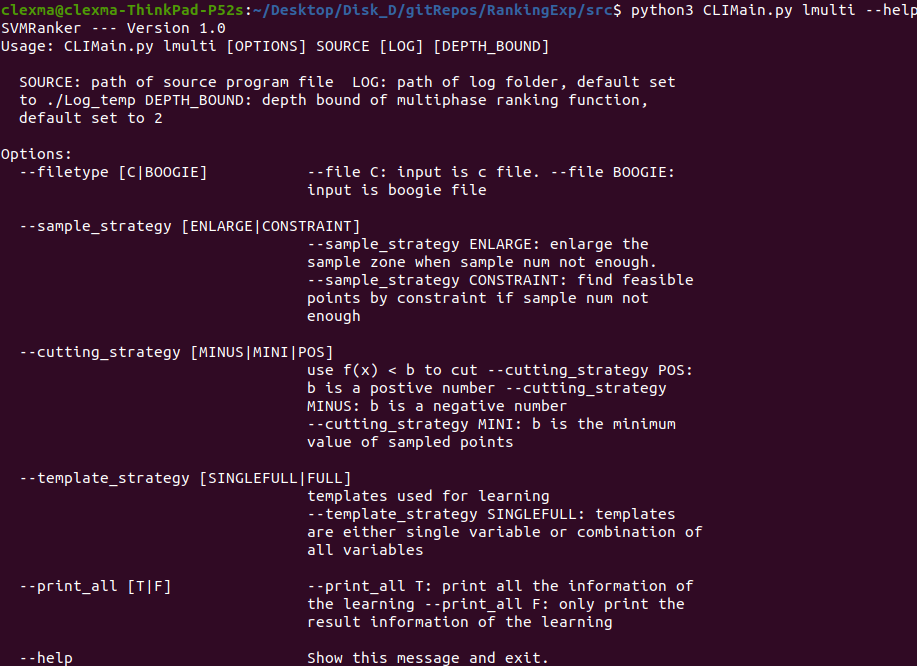
\includegraphics[scale=0.36]{2.png}
\end{center}

\end{frame}

\begin{frame}\frametitle{Tool Demo}
\begin{center}
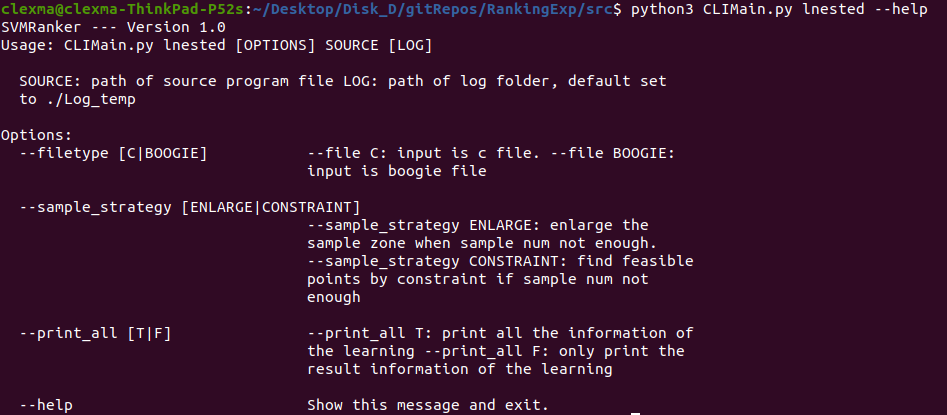
\includegraphics[scale=0.34]{3.png}
\end{center}

\end{frame}
\begin{frame}\frametitle{Tool Demo}
\begin{center}
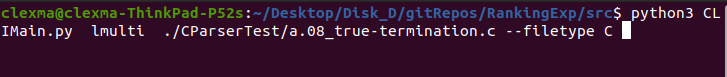
\includegraphics[scale=0.4]{5.png}

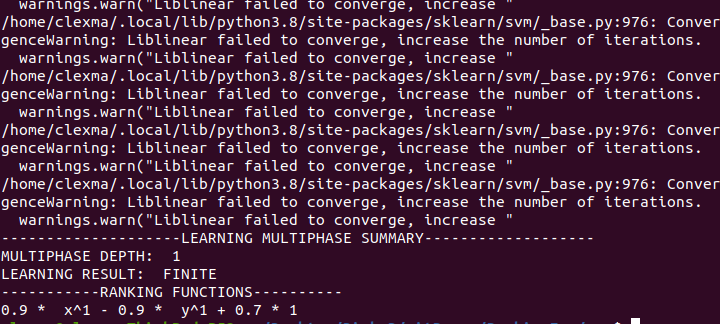
\includegraphics[scale=0.4]{4.png}
\end{center}
\end{frame}

\begin{frame}\frametitle{TODOs}
\begin{itemize}
\item Use translation of C to Boogie in Ultimate.

\item Use AST instead of Python array for program input.

\item Recurrent Set.
\end{itemize}
\end{frame}
\end{document}
